\section{Durchführung}
\label{sec:Durchführung}
Der in diesem Versuch verwendete Aufbau ist in \autoref{fig:Aufbau} dargestellt.
\begin{figure}[H]
    \centering
    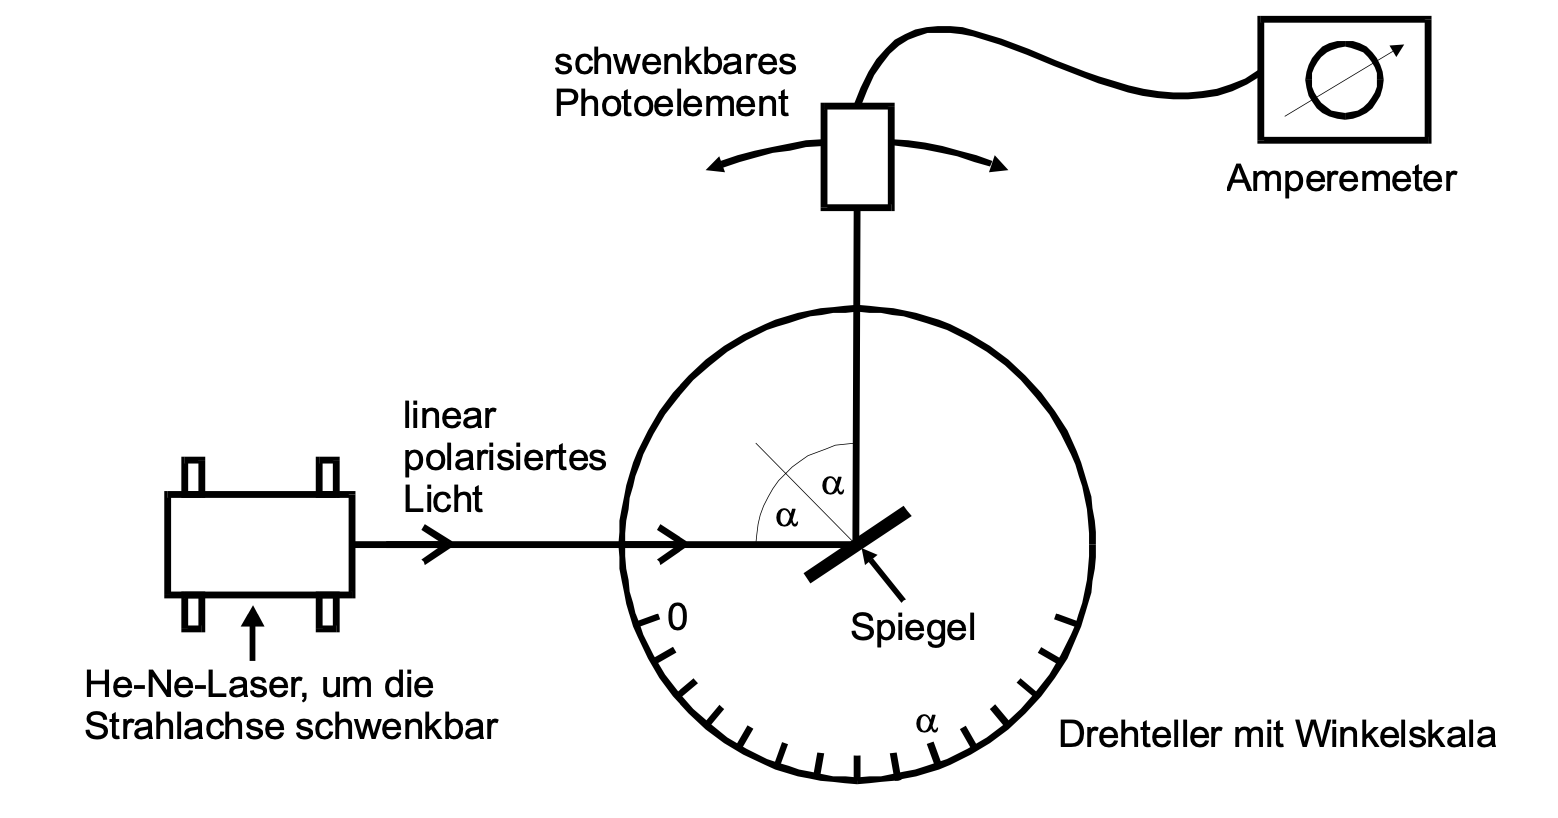
\includegraphics[height=6cm]{content/pics/Aufbau.png}
    \caption{Schematischer Aufbau des Experimentes \cite{v407}.}
    \label{fig:Aufbau}
\end{figure}
Der verwendete Laser emmittiert kein polarisiertes Licht, weswegen zwischen Laser und
Spiegel ein Polarisationsfilter gesetzt wird. Der drehbare Spiegel ist im Detail in 
\autoref{fig:Spiegel} gezeigt.
\begin{figure}[H]
    \centering
    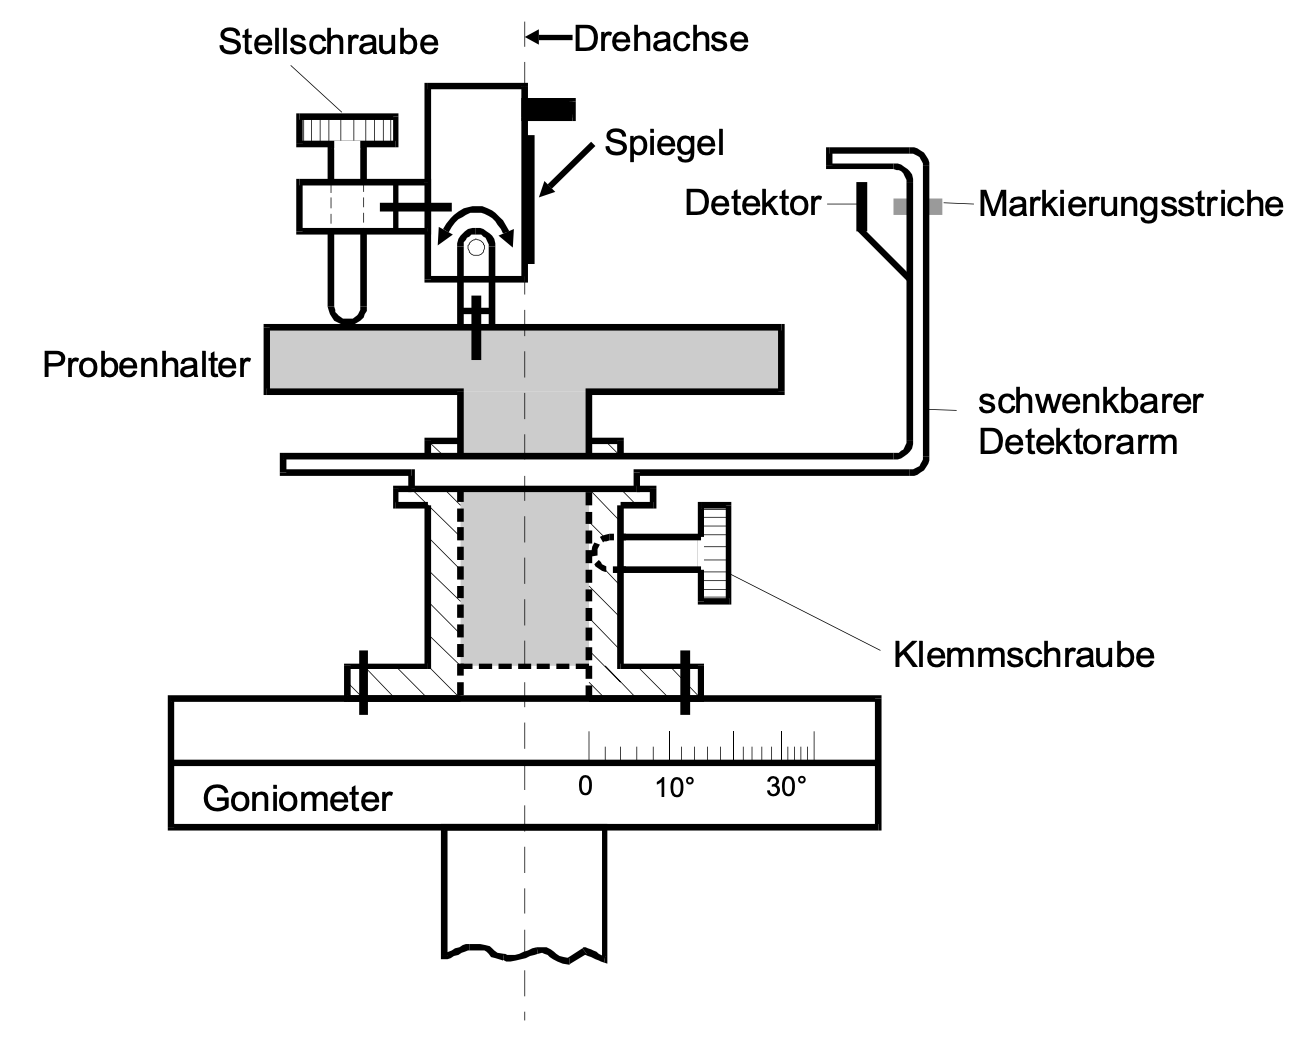
\includegraphics[height=6cm]{content/pics/Goniometer.png}
    \caption{Skizze des verwendeten drehbaren Spiegels mit Goniometer \cite{v407}.}
    \label{fig:Spiegel}
\end{figure}

Bevor die eigentliche Messung starten kann, wird die Messapparatur kalibriert.
Dafür wird
